%Balíčky
\documentclass[a4paper,11pt,twoside]{article}
\usepackage[utf8]{inputenc} %kodovani, abychom mohli jednoduse psat diakriticka pismena
\usepackage[czech]{babel}
\usepackage{pifont}
\usepackage{graphicx} %pro vkladani obrazku
\usepackage{color}
\usepackage{fancyhdr} %zahlavi a zapati
\usepackage{ifpdf}
\usepackage{amssymb}
\usepackage{booktabs}
\usepackage{subfigure}
\usepackage{titlesec}
\usepackage[multiple]{footmisc}
\usepackage[final]{pdfpages}    % pro vkládání PDF souborů
\usepackage{pdflscape}   % pro sazbu stránek naležato
\usepackage{color}       % pro zvýraznění textu barvou
\usepackage{multirow} 
\usepackage{amsmath}
\usepackage{sectsty}
\usepackage[justification=centering]{caption}
\usepackage[top=1.5cm, left=3cm, right=3cm, bottom=2cm, headheight=26pt, includeheadfoot]{geometry}
\usepackage[colorlinks=false,urlcolor=black]{hyperref}
\usepackage{xcolor}
\usepackage{listings}
\hypersetup{
    colorlinks=true,
    linkcolor=black,
    filecolor=black,      
    urlcolor=black,
    citecolor=black
}
\allsectionsfont{\rmfamily} 

\sectionfont{\huge}
\subsectionfont{\LARGE}
\subsubsectionfont{\Large}

\def\author{Autoři: Bc. Linda Kladivová, Bc. Jana Špererová}
\def\nazevprace{GEOMETRICKÉ VYHLEDÁVÁNÍ BODU}

\begin{document}
\setcounter{page}{1}  % nastaví čítač stránek od stránky Úvod na stránku č. 7
\sloppy
\setlength{\parskip}{1pt}


%%  ÚVODNÍ STRÁNKA %%%%%%%%%%%%%%%%%%%%%%%%%%%%%%%%%%%%%%%%%%%%%%

\pagestyle{empty} % vypne číslování stránek na úvodní straně

\begin{center}
\renewcommand{\baselinestretch}{1.35} %zvetseni mezery mezi radky

\LARGE
\textsc{České vysoké učení technické v~Praze} \\
\textsc{Fakulta stavební} \\

\bigskip

\large
\textsc{PROGRAM GEODÉZIE A KARTOGRAFIE} \\
\textsc{OBOR GEOMATIKA} \\

\vspace{10ex}

\begin{figure}[hbt!] %vlozeni loga
\begin{center}

\includegraphics[width=7cm]{pictures/symbol_cvut_konturova_verze_cb.pdf} 
\end{center}
\end{figure}

\vspace{20ex}

\large
\textsc{\nazevprace} \\
\smallskip


\vspace{6ex}

\normalsize
\textsc{\author} \\
\bigskip
\normalsize
\textsc{Předmět: Algoritmy digitální kartografie a GIS} \\

\end{center}


%% 2. STRÁNKA OBSAHUJE ZADÁNÍ
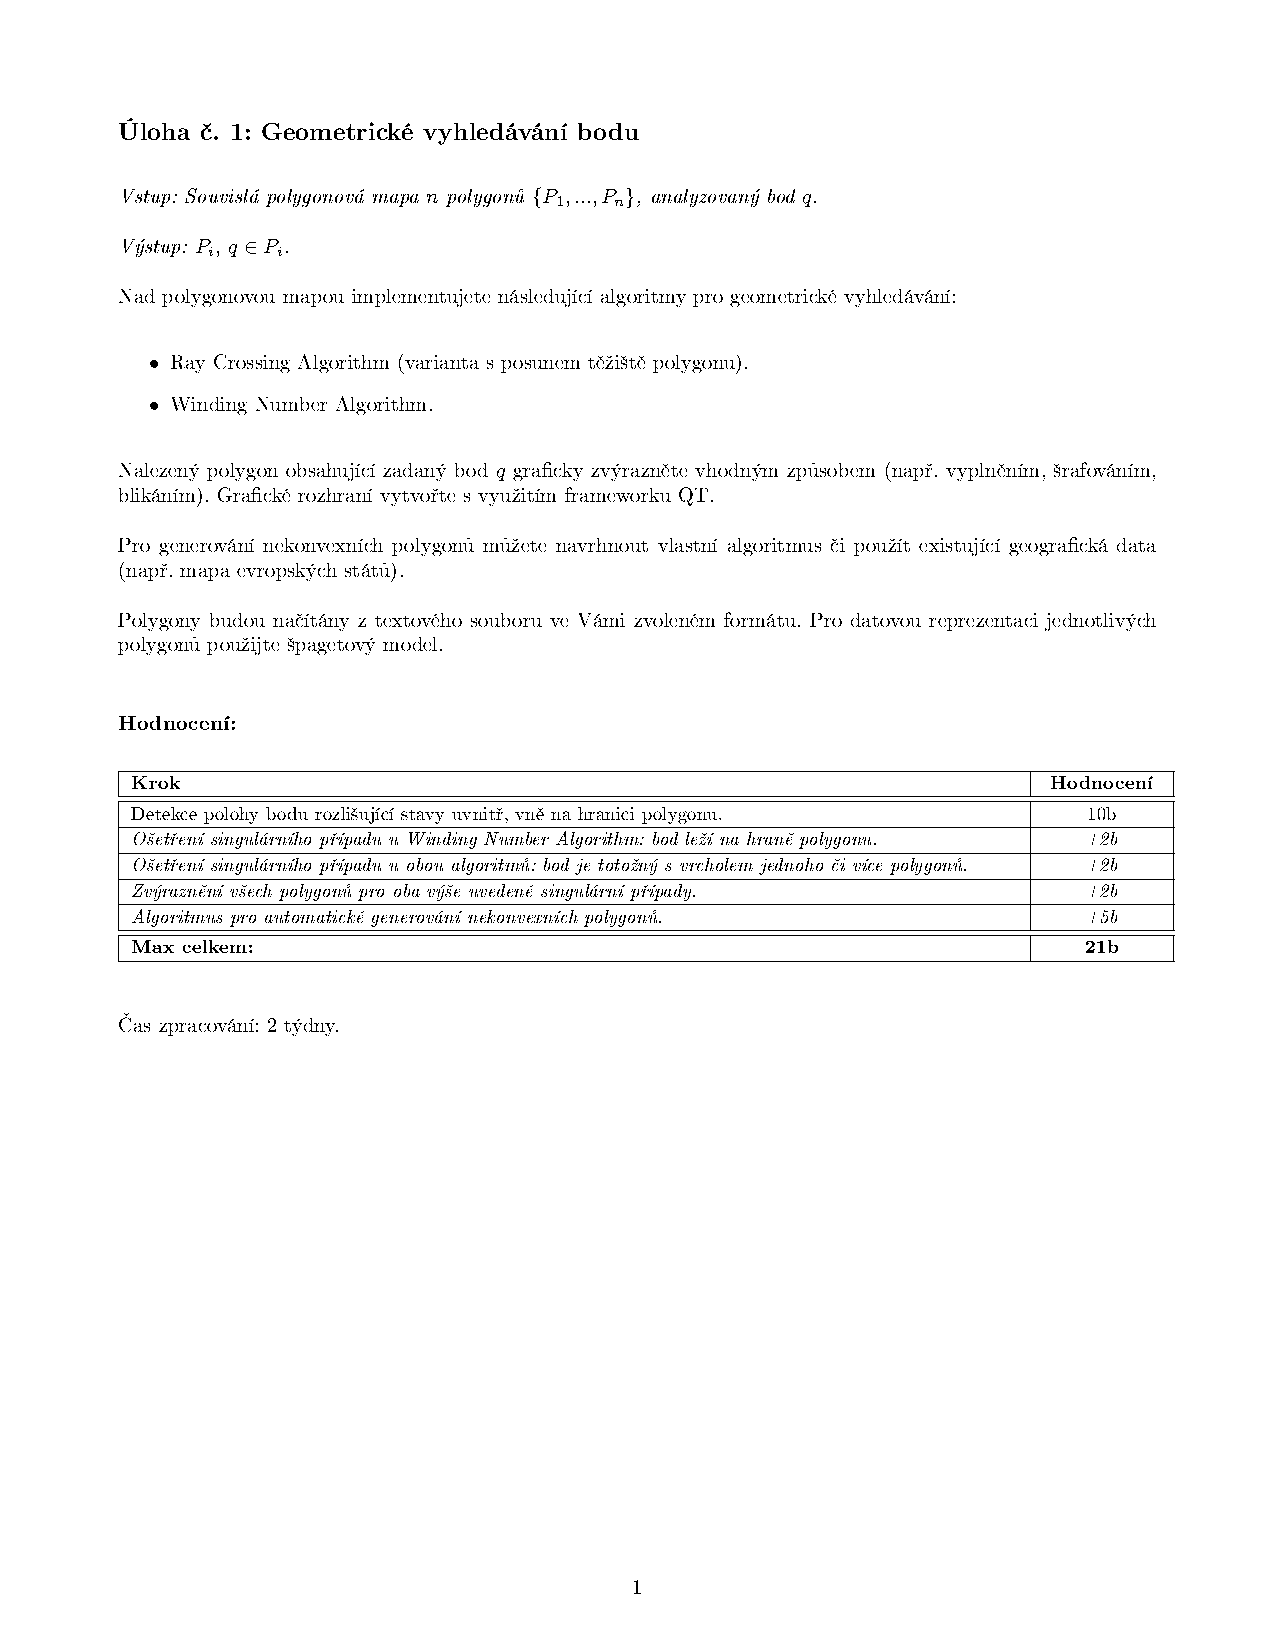
\includepdf{pictures/adkcv1}


%% 3. a 4. STRÁNKA = OBSAH A SEZNAM OBRAZKU %%%%%%%%%%%%%%%%%%%%%%%%%%%%%%%%%%
\renewcommand{\baselinestretch}{1.35} %zvetseni mezery mezi radky
\newpage
\tableofcontents %obsah

\newpage
\listoffigures %seznam obrázků
%\listoftables %seznam tabulek

\thispagestyle{empty}
\newcommand{\obrazek}[1]{(viz obr. \ref{#1})} %specialni reference na obrazek

\newpage
\pagestyle{fancy}

%% NASTAVENI VZHLEDU STRANEK (ZAHLAVI A ZAPATI)

% zajistí, že se názvy kapitol a sekcí nebudou sázet velkými písmeny
\renewcommand{\sectionmark}[1]{\markright{\ #1}}

\fancyhf{} % smaže aktuální nastavení záhlaví a zápatí
\renewcommand{\headrulewidth}{0.4pt} % vrchní linka
\renewcommand{\footrulewidth}{0.4pt}  %  spodní linka
\addtolength{\voffset}{-0.4cm}

 %záhlaví
\fancyhead[LE, LO]{{
\includegraphics[width=1cm]{pictures/symbol_cvut_konturova_verze_cb.pdf} }
   {\textsc{\small {ČVUT v Praze}} }} %logo skoly
\fancyhead[RE, RO]{\nouppercase{\rightmark}}
   
 %zápatí
\fancyfoot[RO, LE]{{\textsc{\small \thepage}}}

\fancypagestyle{plain}{
  \fancyhead{} % na prázdných stránkách nechci záhlaví
  \renewcommand{\headrulewidth}{0pt} % ani linku
}


%% -------<<< 1. KAPITOLKA = Popis a rozbor problému >>>-------\\%%

\newpage
\pagestyle{fancy}
\fancyhead[RE, RO]{\fancyplain{}{\small \sl{POPIS A ROZBOR PROBLÉMU}}}

\vspace*{-1cm}
\section{Popis a rozbor problému}
\noindent
\large
Formulace problému je velmi přímočará. V rovině je dána množina bodů, které tvoří vrcholy mnohoúhelníků, a je dán bod q. Cílem je vyřešit tzv. Point Location Problem (PLP), tedy najít takový mnohoúhelník P, který bod q obsahuje. Tento problém je velmi významný, jelikož velice často potřebujeme znát svoji polohu vůči jiným objektům. Přústupů řešení tohoto problému je hned několik a závisí na tvaru polygonu, který může být ve speciálním případě konvexní, ale nejčastěji bývá nekonvexní. \\
\indent Mnohoúhelník, který je konvexní, splňuje podmínku, že všechny jeho vnitřní úhly jsou konvexní, tedy musí být menší nebo rovny $180^\circ$. Dále platí, že všechny body na úsečkách, jejichž krajní body leží uvnitř polygonu, jsou také uvnitř polygonu. Další vlastností je, že všechny strany konvexního mnohoúhelníku leží v tzv. opěrné polorovině. U nekonvexního typu toto neplatí, což je zřejmé z obrázku \ref{fig:srovnani_konvex}.

\vspace{0.2cm}
\begin{figure}[hbt!] 
\begin{center}
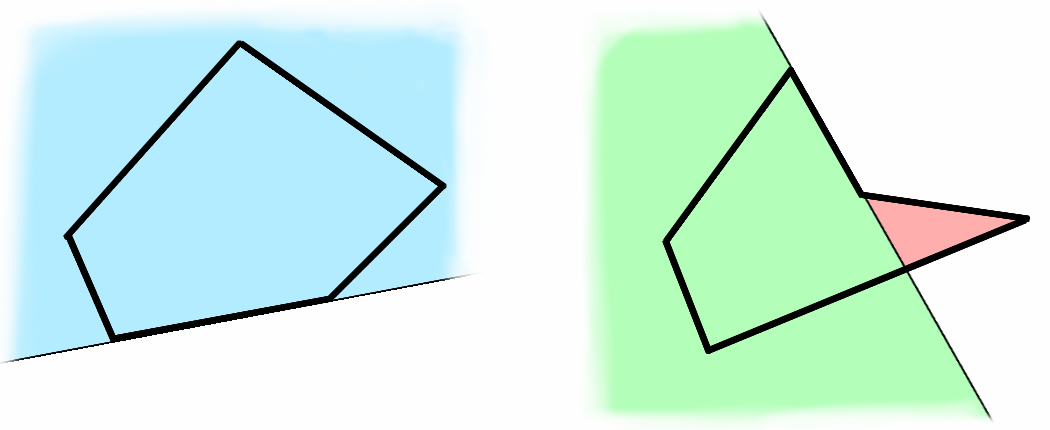
\includegraphics[width=15cm]{pictures/Srovnani-konvex.png} 
\caption[Srovnání konvexního a konkávního mnohoúhelníku]{Srovnání konvexního a konkávního mnohoúhelníku \cite{srovnani_konvex}}
\label{fig:srovnani_konvex}
\end{center}
\end{figure}
\vspace{-0.4cm}

\noindent
\large
Výsledkem testu polohy bodu a mnohoúhelníku může být několik různých vzájemných poloh:
\begin{itemize}
		\item bod q leží uvnitř testovaného polygonu P,
		\item bod q leží mimo testovaný polygon P,
		\item bod q leží na hraně testovaného polygonu P,
		\item bod q je identický s některým z vrcholů polygonu P.
\end{itemize}

Pro testování vzájemné polohy bodu vůči polygonu existuje několik metod. V této úloze je naprogramována metoda Ray Crossing Algorithm (varianta s posunem těžiště polygonu) a metoda Winding Number Algorithm.

\subsection{Údaje o bonusových úlohách}
\large
\noindent Kromě implementace výše zmíněných algoritmů pro geometrické vyhledávání bodu nad polygonovou mapou, byl ošetřeno několik singulárních případů. U Winding Number Algorithm byl ošetřen případ, kdy bod leží na hraně polygonu. U obou algoritmů došlo k podchycení případu, kdy bod je totožný s vrcholem jednoho či více polygonů. Pro uvedené singularity bylo provedeno zvýraznění polygonů zelenou barvou. Zároveň byl naprogramován algoritmus pro automatické genererování nekonvexních polygonů. 

%% -------<<< 2. KAPITOLA = Popis použitých algoritmů >>>-------\\%%

\fancyhead[RE, RO]{\fancyplain{}{\small \sl{POPIS POUŽITÝCH ALGORITMŮ}}}
\section{Popis použitých algoritmů}
\noindent
\large
Cílem této úlohy je vytvořit aplikaci, která po zadání příslušného bodu q určí polygon P, do kterého zadaný bod přísluší. Při volbě metody je vždy nutné se zamyslet nad typem vstupních a výstupních dat a nad časovou náročností. \\
\indent Řešení pro konvexní polygony je nejčastěji realizováno opakovaným testem polohy bodu q vůči každé hraně mnohoúhelníku P (half-plane test) nebo pomocí Ray Crossing Algorithm (paprskovitého algoritmu). Test polohy bodu q vůči hranám mnohoúhelníku P je princip, který ale nelze aplikovat na nekonvexní polygony. \\
\indent K řešení této úlohy pro nekonvexní algoritmy jsou používány dva algoritmy: paprsový (Ray algorithm) a metoda ovíjení (Winding algorithm). Oba tyto přístupy převádí problém na opakované určení bodu vzhledem k mnohoúhelníku. Rozdílnou technikou řešení planární dělení roviny, což je jiná skupina algoritmů daleko mocnější, ale náročnější na implementaci. Do této skupiny patří například Metoda pásů, Line Sweep Algorithm či metoda trapezoidálních map.

\subsection{Ray Crossing Algorithm}
\large
\noindent Ray Crossing Algorithm primárně slouží pro určení vztahu bod versus konvexní mnohoúhelník.  Je však možné ho naprogramovat i pro nekonvexní polygony, což bude náš případ. Podstata algoritmu spočívá v tom, že ze zájmového bodu vedeme polopřímku a počítáme její průsečíky s hranami polygonu. Tento algoritmus je o řád rychlejší než Winding algoritmus, problémem jsou však singularity. Princip paprskového algoritmu je zřejmý z obrázku \ref{fig:ray}.\\

\vspace{0.2cm}
\begin{figure}[hbt!] 
\begin{center}
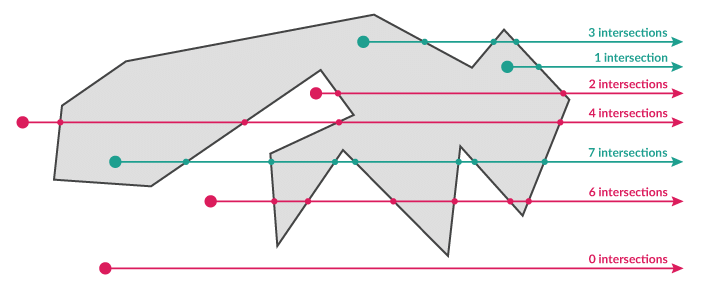
\includegraphics[width=15cm]{pictures/ray.png} 
\caption[Princip paprskového algoritmu]{Princip paprskového algoritmu \cite{ray}}
\label{fig:ray}
\end{center}
\end{figure}
\vspace{-0.4cm}

\noindent Počet průsečíků paprsku r s hranou polygonu označme M. Platí, že:
\begin{itemize}
\item pokud je M liché: bod náleží polygonu P $(q\in P)$ ,
\item pokud je M sudé: bod nenáleží polygonu P $(q { \not\in } P)$ .
\end{itemize}

\subsubsection{Implementace algoritmu (varianta s redukcí)}
\begin{enumerate}
\item Nastavení počtu průsečíků rovno nule:  $ intersects = 0 $ 
\item Redukce souřadnic všech bodů polygonu vůči souřadnicím bodu q (lokální souřadnicový systém (q, x', y'))
\item Test podmínky:  $if(y'_i > 0)\&\&(y'_{i-1} <= 0)\|(y'_{i-1} > 0)\&\&(y'_{i} <= 0)  $ 
\item Při splnění podmínky provedení:  $ x'_m = (x'_i y'_{i-1} - x'_{i-1} y'_i ) / (y'_i - y'_{i-1})$ 
\item Pokud $x'_m > 0$, zvýšení počtu průsečíků o jeden: $ intersects = intersects +1$
\item Určení, zda je počet průsečíků sudý či lichý: $if (intersect\%2) = 0$, pak: $q\in P$
\item V opačném případě: $q {\not \in} P$
\end{enumerate}

\newpage
\vspace*{-1cm}
\subsection{Winding Number Algorithm}
\large
\noindent Tento algoritmus je také nazýván Metoda ovíjení. Půjdeme postupně po vrcholech polygonu P a budeme sčítat nebo odečítat úhly mezi daným bodem q a vrcholy P (po směru hodinových ručiček přičítáme, proti směru odečítáme). Pokud je výsledný úhel roven 2$\pi$, byl dokončen celý kruh, lze tedy prohlásit, že bod q náleží polygonu P. Pokud je výsledný úhel roven 0, bod q polygonu P nenáleží. Princip Winding algoritmu je zřejmý z obrázku \ref{fig:winding}.

\vspace{0.2cm}
\begin{figure}[hbt!] 
\begin{center}
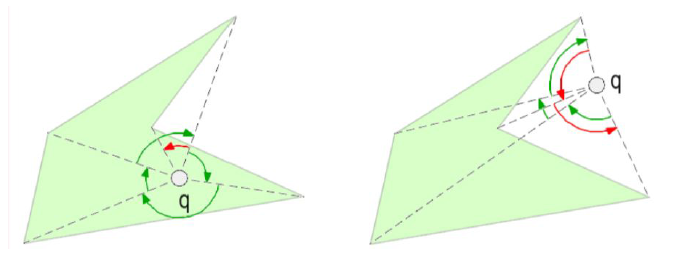
\includegraphics[width=15cm]{pictures/winding.png} 
\caption[Princip Winding algoritmu]{Princip Winding algoritmu \cite{winding}}
\label{fig:winding}
\end{center}
\end{figure}
\vspace{-0.4cm}

\noindent Při této metodě je zapotřebí počítat Winding Number $\Omega$. Pro toto číslo platí, že je rovno sumě všech rotací $\omega$ proti směru hodinových ručiček, které průvodič opíše nad všemi body: 
$$ 
\Omega = \frac{1}{2\pi} \sum_{i=1}^n \omega_i
$$.

\noindent Platí, že pokud je úhel $\sphericalangle p_i, q, p_{i+1}$ orientován ve směru hodinových ručiček, pak $\omega_i > 0$.
Naopak pokud je úhel $\sphericalangle p_i, q, p_{i+1}$ orientován proti směru hodinových ručiček, pak $\omega_i < 0$. V závislosti na výsledné hodnotě $\Omega$ lze rozhodnout o poloze bodu q vůči polygonu P:

\begin{itemize}
\item pokud je $\Omega = 1$, platí $q \in P$, 
\item pokud je $\Omega = 0$, pak platí $q { \not \in } P$.
\end{itemize}

\newpage
\vspace*{-1cm}
\subsubsection{Implementace metody}
\begin{enumerate}
\item Nastavení výchozího úhlu $\omega = 0$ , volba tolerance $\epsilon$ : $\omega = 0, \epsilon = 1e-6$
\item Určení úhlu: $\omega_i = \sphericalangle p_i, q, p_{i+1}$
\item Určení orientace $o_i$ bodu q ke straně $p_i, p_{i+1}$
\item Volba podmínky - pokud bod vlevo: $\omega = \omega + \omega_i$, v opačném případě: $\omega = \omega - \omega_i$
\item Volba podmínky - pokud rozdíl: $|(|\omega| - 2\pi)| < \epsilon$, pak platí: $q \in P$, v opačném případě:  $ q { \not \in } P $
\end{enumerate}

\subsection{Generování nekonvexního polygonu}
Uživatel si nejprve zadá počet vrcholů polygonu, jež bude poté automaticky vygenerován. Pokud zvolí počet vrcholů 1,2 nebo 3 je zobrazena chybová hláška. Počet vrcholů polygonu musí být nejméně 4, aby mohl být výsledný obrazec nekonvexní. 
Souřadnice náhodných bodů jsou redukovány pomocí funkce modulo, aby bylo zajištěno zobrazení bodů ve vykreslovacím widgetu.\\
\indent Uvnitř kódu je náhodně generováno (n - 1) bodů, jelikož jako n-tý bod je vygenerován střed všech vygenerovaných bodů. Od tohoto cetrálního bodu jsou poté vypočteny směrníky na všechny další body, díky čemuž mohly být body v polygonu seřazeny ve směru hodinových ručiček. Díky výpočtu směrníku je výsledný polygon topologicky korektní, ale je nutné brát ohled na kvadranty arcus tangens.

\subsubsection{Implementace metody}
\begin{enumerate}
\item Náhodné vygenerování (n-1) bodů:  $x_{pi} = rand \% 1000; y_{pi} = rand \% 600$.
\item Vygenerování centrálního bodu jakožto průměru z již vygenerovaných souřadnic bodů.
\item Výpočet směrníků z centrálního bodu na jednotlivé body v závislosti na osách daného zobrazovacího okna.
\item Určení kvadrantu a správný přepočet úhlu.
\item Seřazení bodů v polygonu ve směru hodinových ručiček, tedy od nejmenšího směrníku.
\end{enumerate}

%% -------<<< 3. KAPITOLKA = Problematické situace a jejich rozbor >>>-------\\%%
\newpage
\vspace*{-1cm}
\fancyhead[RE, RO]{\fancyplain{}{\small \sl{PROBLEMATICKÉ SITUACE A JEJICH ROZBOR}}}
\section{Problematické situace a jejich rozbor}
\subsection{Ray Crossing Algorithm}
\large
Při programování tohoto algoritmu bylo řešeno několik problematických situací, tzv. singularit. K singularitě zde může dojít tehdy, pokud bod leží na hraně polygonu či pokud je bod identický s některým z vrcholů polygonu. Z tohoto důvodu se využívá upravená varianta Ray Crossing Algorithm, kdy je nejprve provedena redukce souřadnic bodů polygonu k zájmovému bodu a dále se testuje souřadnice y vybraného bodu polygonu a bodu předcházejícího. Počítají se pouze průsečíky M ležící v 1. kvadrantu upraveného souřadnicového systému, tedy souřadnice x bodu M musí být kladná. Problematické singulární situace můžeme vyjádřit následovně:
\begin{itemize}
\item Bod q je totožný s vrcholem polygonu P:  $  q [x_q, y_q] = p_i [x_i, y_i] $ 
\item Bod q leží na některé z hran AB polygonu P:   $  q \in \overrightarrow{AB} $ 
\end{itemize}

\noindent První případ byl ošetřen porovnáním souřadnic bodu q a souřadnic bodu polygonu (tolerance totožnosti byla zvolena 1e-6). Druhý případ byl ošetřen pomocí funkce getPointLinePosition. Pokud bod náležel hraně polygonu či se nalézal ve vrcholu polygonu, byla návratová hodnota rovna -1. V takovém případě byl bod q vyhodnocen, že se v polygonu P nachází.

\subsection{Winding Number Algorithm}
\large
K singulárním případům dochází pouze v případě, že $q \approx p_i$, tedy v případě že zájmový bod je téměř identický s některým z vrcholů polygonu. Pokud tomu nastane, vyhodnotí se funkce tak, že bod leží v obou polygonech. Problematické singulární situaci můžeme vyjádřit následovně:

\begin{itemize}
\item Bod q je totožný s vrcholem polygonu P:  $  q [x_q, y_q] \approx p_i [x_i, y_i] $ 
\end{itemize}

\noindent Tento případ byl ošetřen porovnáním souřadnic bodu q a souřadnic bodu polygonu (tolerance totožnosti byla zvolena 1e-6).

%% -------<<< 4. KAPITOLA = Vstupní  data >>>-------\\%%
\newpage
\fancyhead[RE, RO]{\fancyplain{}{\small \sl{VSTUPNÍ A VÝSTUPNÍ DATA}}}

\vspace*{-1cm}
\section{Vstupní data}
Vstupní data tvoří analyzovaný bod q a textový soubor s body jednotlivých polygonů. Vstupem může také být automaticky vygenerovaný nekonvexní polygon.
\begin{itemize}
\item Bod q je vložen uživatelem po ztisknutí tlačítka v grafickém okně aplikace.
\item Souvislá mapa polygonů je ve formátu txt a obsahuje body jednotlivých polygonů. Má strukturu
[číslo bodu, souřadnice X, souřadnice Y]. Soubor je seřazen od bodu č. 1 po n-tý bod polygonu. Jednotlivé body se nejprve uloží do proměnné typu QPointF a následně do proměnné polygonu QPolygonF. Jednotlivé polygony se poté uloží do proměnné typu <std::vector>QPolygonF.
\end{itemize}

%% -------<<< 2. KAPITOLA = Výstupní data >>>-------\\%%
\section{Výstupní data}
Hlavním výstupem této úlohy je grafická aplikace, která umožňuje nahrání textového souboru s body polygonů a následné zobrazení těchto bodů a mnohoúhelníků. Zároveň je možné v aplikaci určit polohu bodu v rámci polygonu pomocí dvou různých metod - Winding algorithm a Ray Crossing algorithm. Dálším výstupem je zelené vyznačení toho polygonu, kterému bod q náleží. V rámci bonusové úlohy lze mezi výstupy zařadit i automatické vygenerování polygonu, který by měl splňovat podmínky nekonvexního mnohoúhelníku. 
\\

%% -------<<< 3. KAPITOLA = Ukázka aplikace >>>-------\\%%
\newpage
\fancyhead[RE, RO]{\fancyplain{}{\small \sl{UKÁZKA APLIKACE}}}

\vspace*{-1cm}
\section{Ukázka aplikace}
\noindent
\large
Do této kapitolky je zahrnuto několik ukázek vytvořené aplikace.

\vspace{0.2cm}
\begin{figure}[hbt!] 
\begin{center}
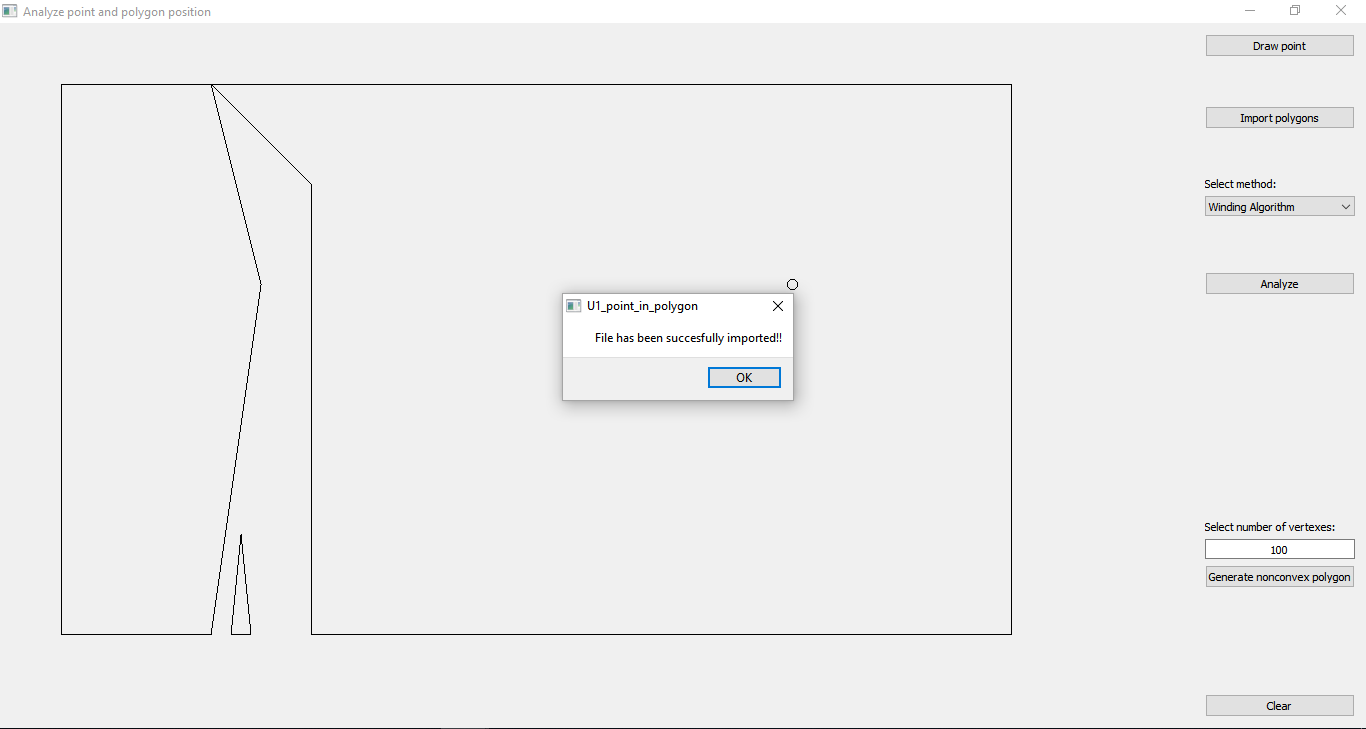
\includegraphics[width=15cm]{pictures/success.png} 
\caption[Úspěšné načtení souboru se souřadnicemi polygonů]{Úspěšné načtení souboru se souřadnicemi polygonů}
\label{fig:success}
\end{center}
\end{figure}

\vspace{0.2cm}
\begin{figure}[hbt!] 
\begin{center}
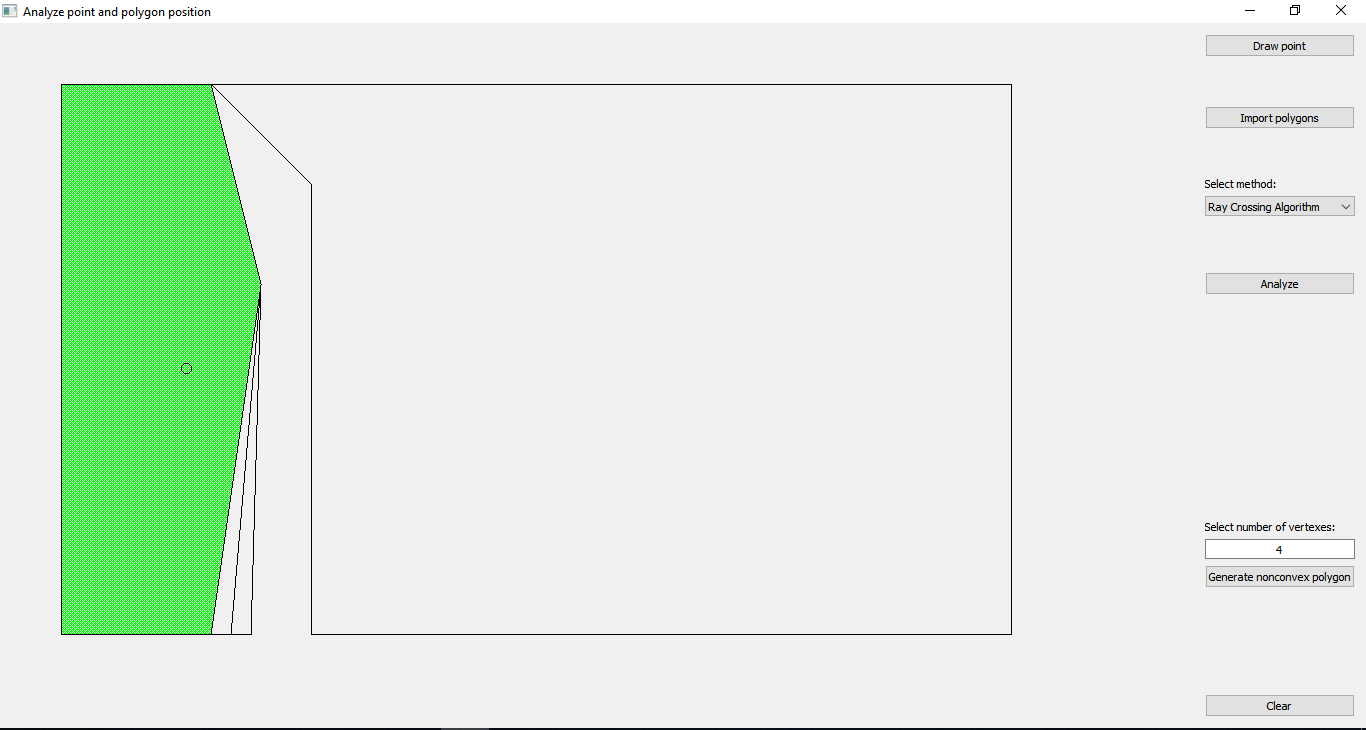
\includegraphics[width=15cm]{pictures/rayinside.png} 
\caption[Analýza Ray Crossing pro bod uvnitř polygonu]{Analýza Ray Crossing pro bod uvnitř polygonu}
\label{fig:rayinside}
\end{center}
\end{figure}

\vspace{0.2cm}
\begin{figure}[hbt!] 
\begin{center}
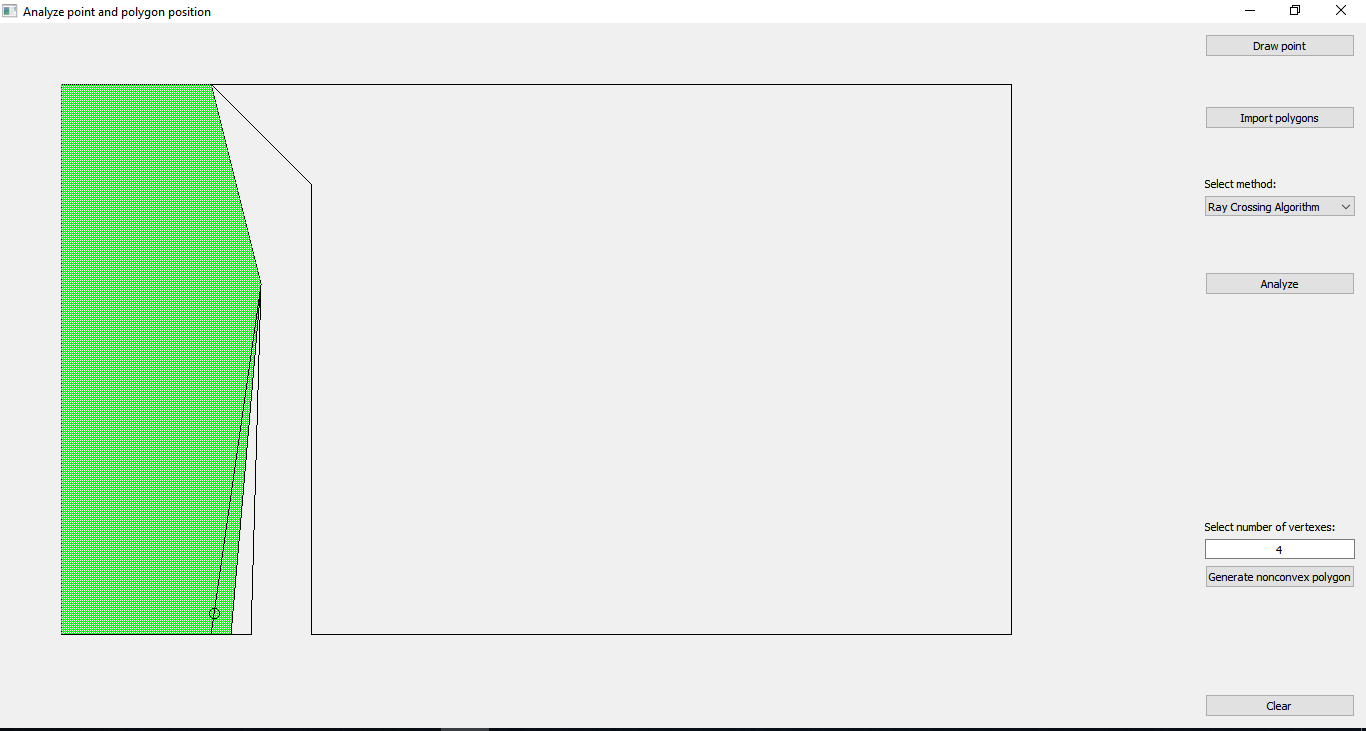
\includegraphics[width=15cm]{pictures/rayonline.png} 
\caption[Analýza Ray Crossing pro bod na hraně polygonu]{Analýza Ray Crossing pro bod na hraně polygonu}
\label{fig:rayonline}
\end{center}
\end{figure}

\vspace{0.2cm}
\begin{figure}[hbt!] 
\begin{center}
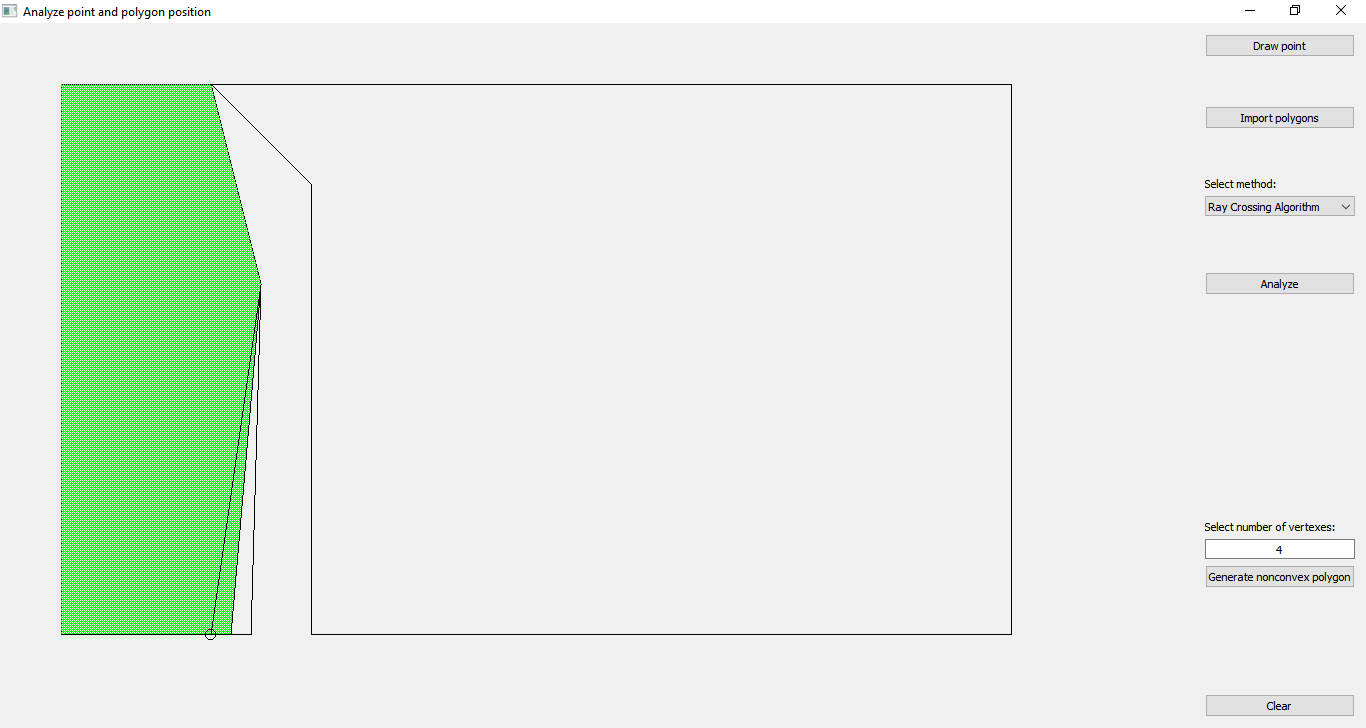
\includegraphics[width=15cm]{pictures/rayonpoint.png} 
\caption[Analýza Ray Crossing pro bod ve vrcholu polygonu]{Analýza Ray Crossing pro bod ve vrcholu polygonu}
\label{fig:rayonpoint}
\end{center}
\end{figure}

\vspace{0.2cm}
\begin{figure}[hbt!] 
\begin{center}
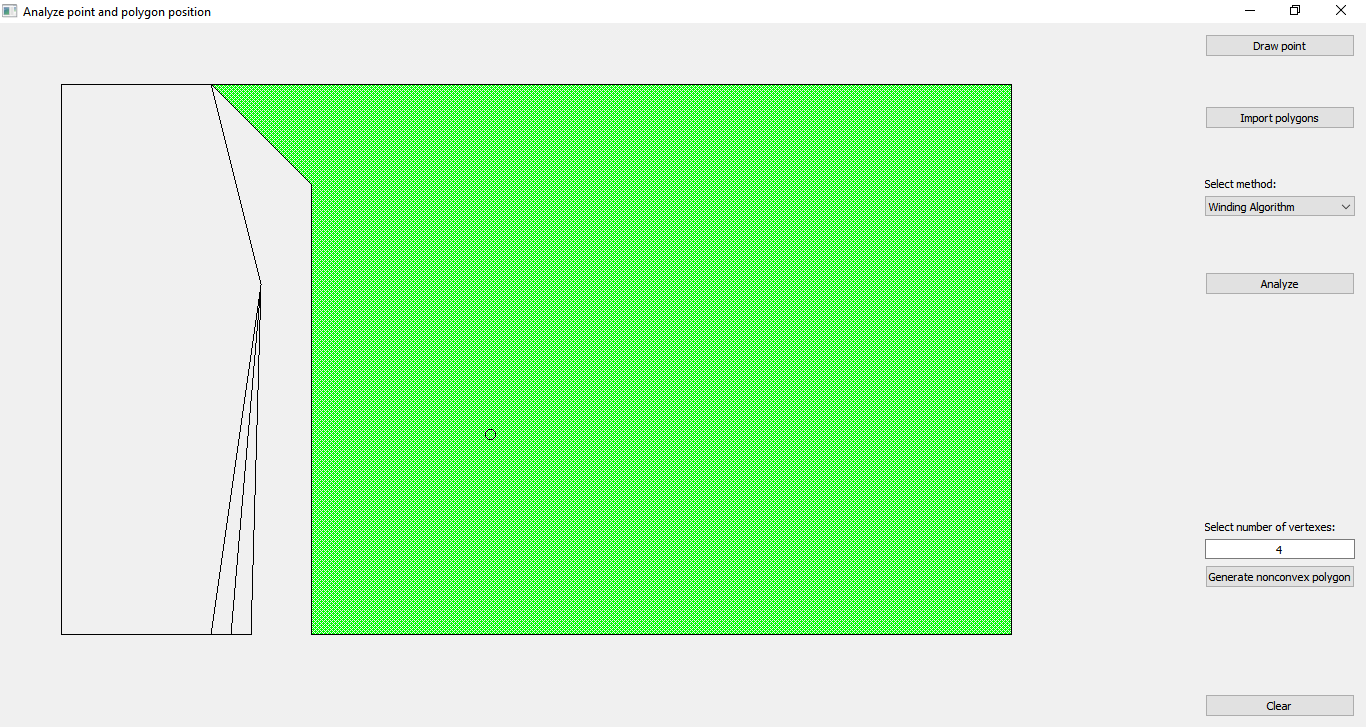
\includegraphics[width=15cm]{pictures/windinside.png} 
\caption[Analýza Winding pro bod uvnitř polygonu]{Analýza Winding pro bod uvnitř polygonu}
\label{fig:windinside}
\end{center}
\end{figure}

\vspace{0.2cm}
\begin{figure}[hbt!] 
\begin{center}
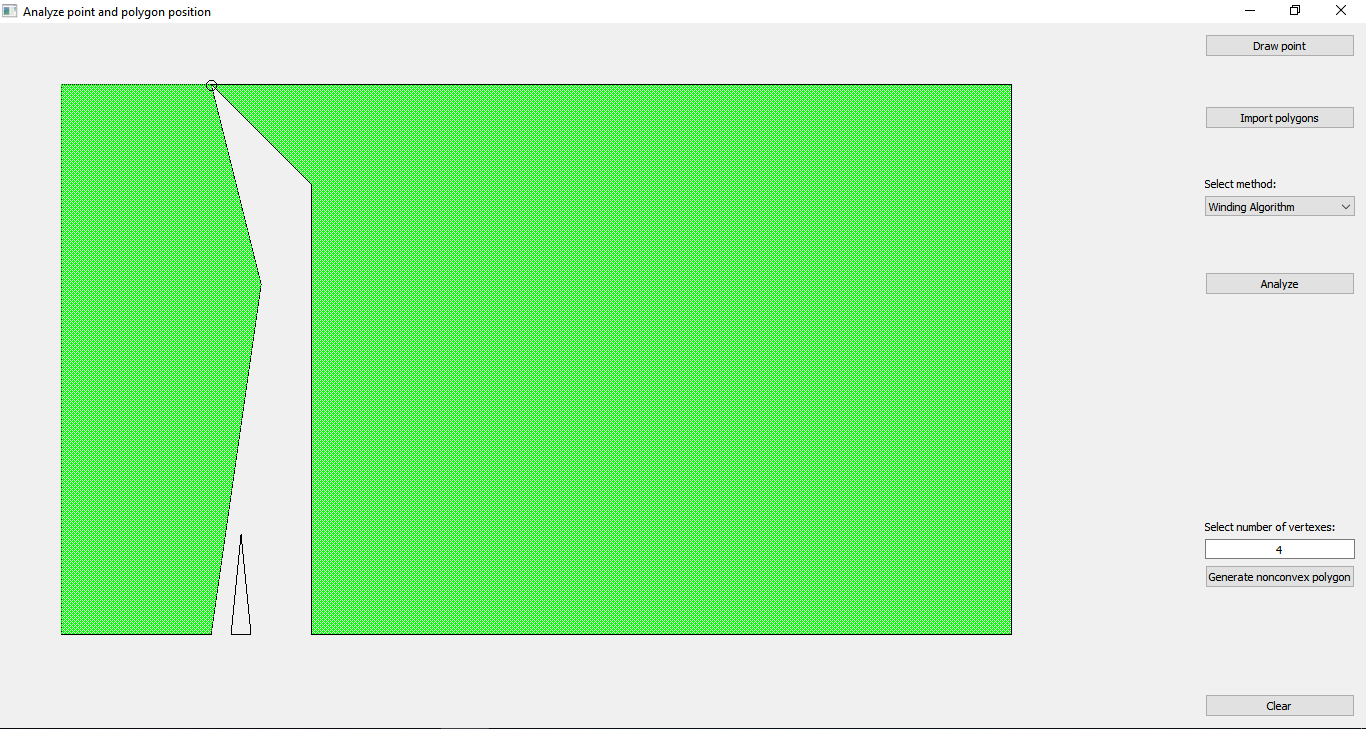
\includegraphics[width=15cm]{pictures/windonpoint.png} 
\caption[Analýza Winding pro bod ve vrcholu polygonu]{Analýza Winding pro bod ve vrcholu polygonu}
\label{fig:windonpoint}
\end{center}
\end{figure}

\vspace{0.2cm}
\begin{figure}[hbt!] 
\begin{center}
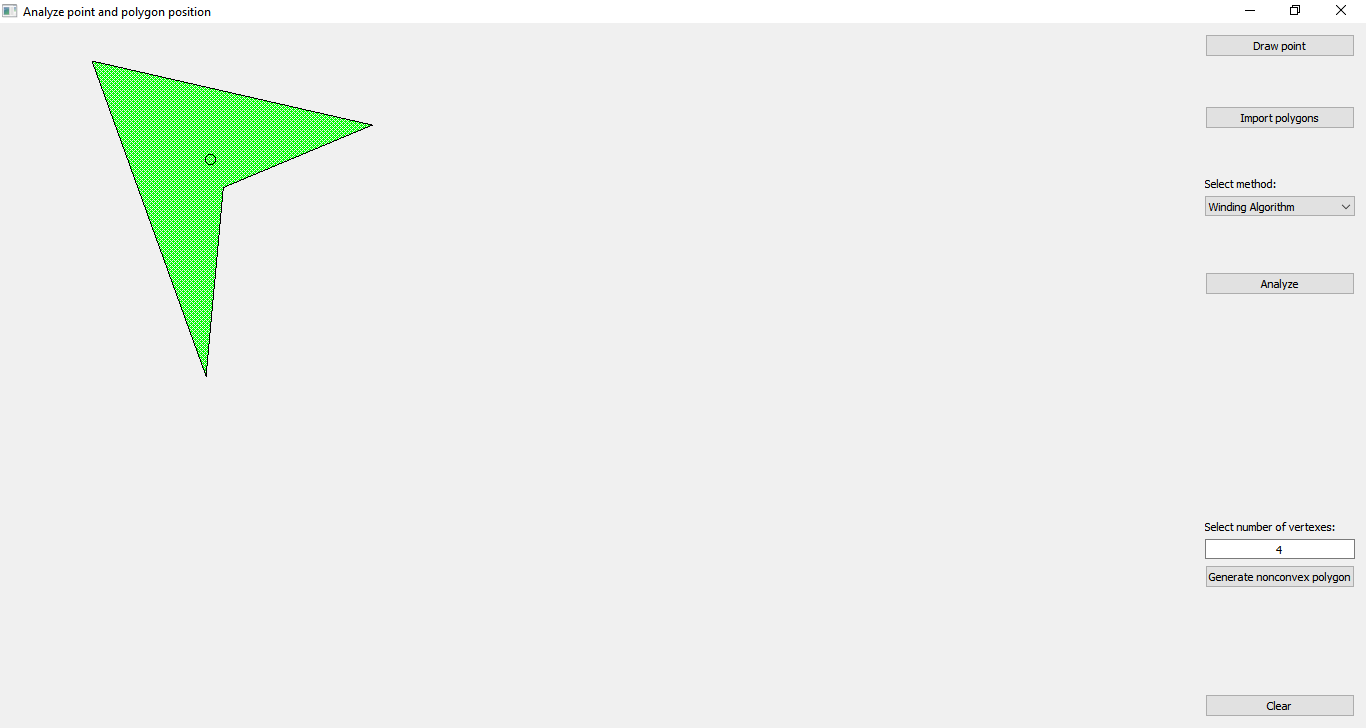
\includegraphics[width=15cm]{pictures/windingongenerated.png} 
\caption[Analýza Winding nad vygenerovaným polygonem]{Analýza Winding nad vygenerovaným polygonem}
\label{fig:windingongenerated}
\end{center}
\end{figure}

\vspace{0.2cm}
\begin{figure}[hbt!] 
\begin{center}
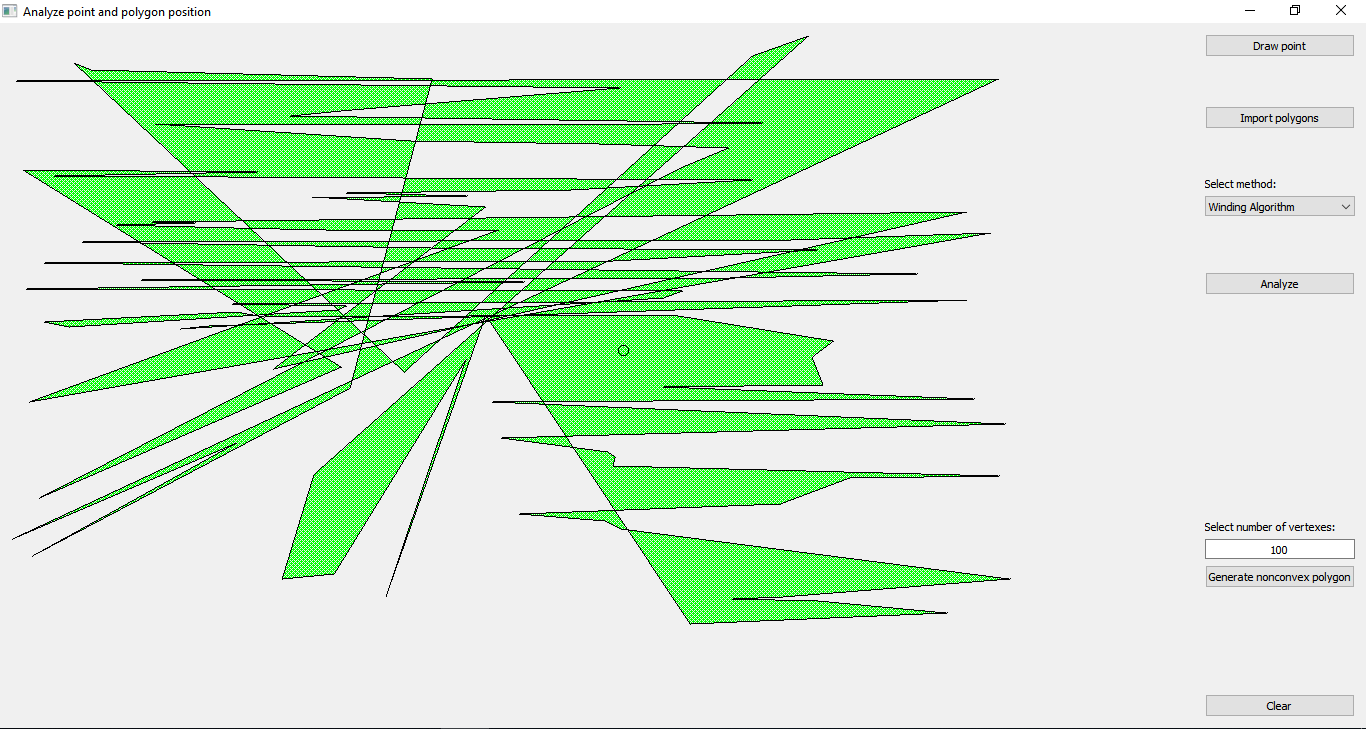
\includegraphics[width=15cm]{pictures/100vertexes.png} 
\caption[Automaticky generovaný nekonvexní polygon se 100 vrcholy]{Automaticky generovaný nekonvexní polygon se 100 vrcholy}
\label{fig:100vertexes}
\end{center}
\end{figure}

\vspace{0.2cm}
\begin{figure}[hbt!] 
\begin{center}
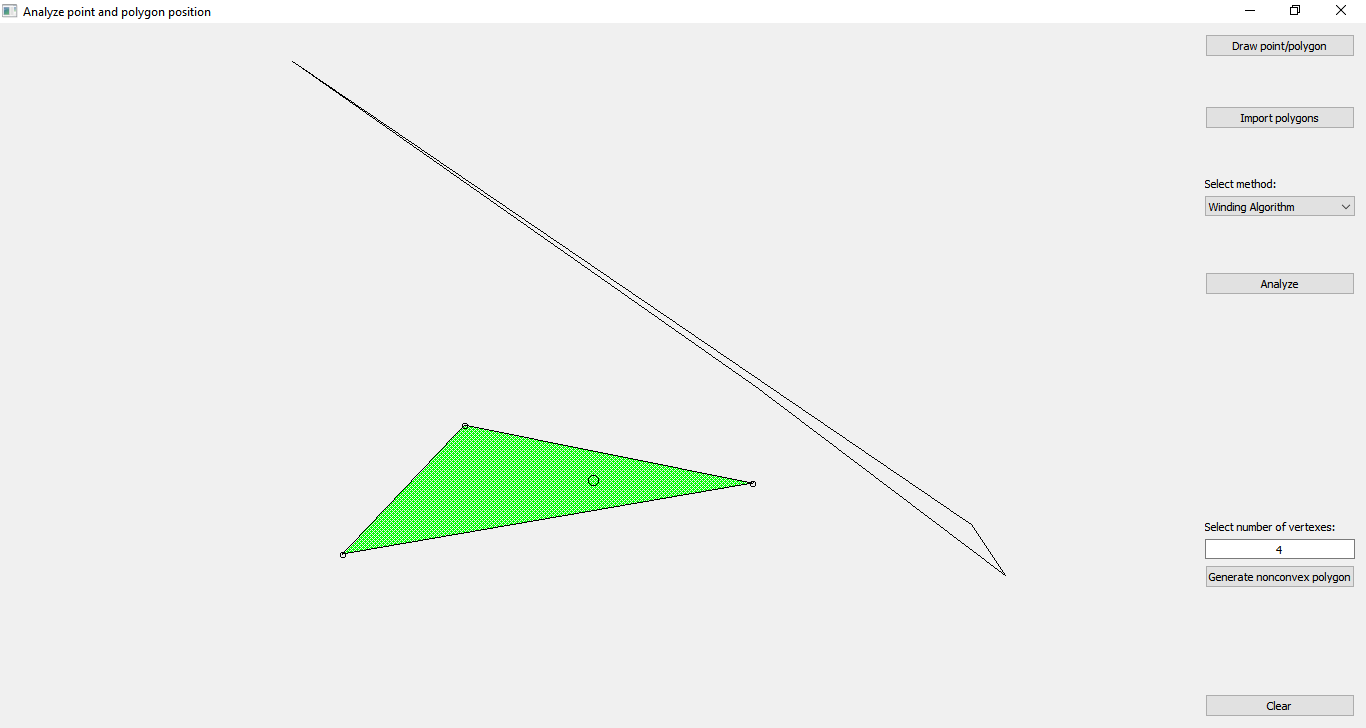
\includegraphics[width=15cm]{pictures/manuallymadepolygon.png} 
\caption[Analýza manuálně a automaticky nakreslených polygonů]{Analýza manuálně a automaticky nakreslených polygonů}
\label{fig:manuallymadepolygon}
\end{center}
\end{figure}

%% -------<<< 4. KAPITOLA = Technická dokumentace >>>-------\\%%

\newpage
\fancyhead[RE, RO]{\fancyplain{}{\small \sl{TECHNICKÁ DOKUMENTACE}}}

\vspace*{-1cm}
\section{Technická dokumentace}
\subsection{Třídy}
V aplikaci se nachází celkem tři třídy Algorithms, Draw a Widget. Každá z těchto tříd má svůj hlavičkový soubor, kde je deklarována spolu se svými metodami, a svůj zdrojový soubor, ve kterém jsou její metody konkrétně definovány.
\subsubsection{Algorithms}
Třída Algorithms obsahuje konstruktor a další čtyři metody, které jsou určeny pro výpočet algoritmů používaných v digitálním GIS. Datové typy u bodu a polygonu byly zvoleny s plovoucí desetinnou čárkou (floating point).\\

\noindent\textbf{int positionPointPolygonRayCrossing(QPointF q, QPolygonF pol)}\\
Jedná se o funkci, která vypočítá polohu bodu vůči polygonu využitím Ray Crossing Algorithm (paprskového algoritmu). Do funkce vstupuje určovaný bod \textit{q} a polygon \textit{P}, vůči kterému je poloha zjišťována. V případě, že výsledná hodnota funkce je rovna \textit{1}, znamená to, že bod leží v polygonu, případně na hraně či vrcholu polygonu -- singulární případy jsou ošetřeny pomocí funkce getPointLinePosition. V ostatních případech leží bod mimo polygon.\\

\noindent\textbf{int positionPointPolygonWinding(QPointF q, QPolygonF pol)}\\
Tato funkce určí polohu bodu vůči polygonu metodou Winding Number Algorithm. Vstupem je určovaný bod \textit{q} a polygon \textit{P}, vůči kterému je poloha určována. Hned na počátku je také zvolena tolerance (minimální hodnota) \textit{eps = 1e-6}. V případě, že výstupem je číslo \textit{0}, bod leží mimo polygon, v případě že \textit{1}, bod leží uvnitř polygonu. Pokud nenastane žádná z těchto uvedených možností, výstupem je hodnota \textit{-1}. Ve funkci je mimo jiné ošetřena singularita, která může nastat v případě, že bod leží na hraně či ve vrcholu. Pokud je výstupem číslo rovno \textit{1}, znamená to, že bod \textit{q} buď leží v některém z vrcholů polygonu \textit{P}, nebo leží na hraně polygonu, což je kontrolováno funkcí getPointLinePosition. \\

\noindent\textbf{int getPointLinePosition(QPointF q, QPointF p1, QPointF p2)}\\
Tato funkce má za úkol určit polohu bodu \textit{q} vůči přímce zadané dvěma body \textit{p1} a \textit{p2}. Z vypočtených vektorů určíme determinant, jehož velikost je stěžejší pro správné určení polohy bodu \textit{q}.  Aby bylo možné s menším rozptylem definovat situaci, kdy bod leží přímo na přímce, byla inicializována tolerance (minimální hodnota) \textit{eps = 1e-6}. Pokud je determinant větší než tato tolerance, bod se nechází v levé polorovině a funkce vrací hodnotu \textit{1}. Pokud je menší, bod se nachází v pravé polorovině a funkce vrací hodnotu \textit{0}.  Pokud nenastane ani jeden z výše uvedených případů, znamená to, že bod leží blízko hrany a výstupem je hodnota \textit{-1}.\\

\noindent\textbf{double getAngle2Vectors(QPointF p1,QPointF p2,QPointF p3, \\ QPointF p4)}\\
V této funkci je pomocí norem a skalárního součinu počítán úhel mezi dvěma hranami zadanými čtyřmi body typu QPoint. Úhel je vypočten jako arcus cosinus poměru skalárního součinu a součinu obou velikostí. Defaultně se v prostředí počítá v radiánech, což bylo ponecháno.

\newpage
\vspace*{-1cm}
\subsubsection{Draw}
Třída Draw dědí od třídy QWidget. Je v ní obsaženo několik metod a také kontruktor, který nastavuje počáteční kursor mimo kreslící okno.\\

\noindent\textbf{void setDrawMode}\\
Po spuštění aplikace je nutné stisknout tlačítko Draw Point pro vykreslení bodu. V případě, že se stiskne tlačítko znovu, je přivolána funkce k tvorbě polygonu. Další možností je importovat polygony ze souboru nebo automaticky generovat náhodné polygonu o předem vybraném počtu vrcholů.\\

\noindent\textbf{void mousePressEvent}\\
V této funkci je v závislosti na hodnotě textit{draw\_mode} vykreslen buď nový bod \textit{q}, nebo nový bod polygonu \textit{P}.\\

\noindent\textbf{void paintEvent}\\
Tato metoda slouží k vykreslení bodu q. Zároveň jsou díky této metodě vykresleny naimportované polygony nebo nakreslený polygon. V metodě je také naprogramováno zvýraznění polygonu, pokud bod \textit{q} leží uvnitř, případně na hraně či ve vrcholu polygonu \textit{P}.\\

\noindent\textbf{void setResult}\\
Metoda, která výsledek analýzy vytvořený po kliknutí na tlačítko Analyze ve třídě Widget, udělá viditelný i pro třídu Draw.

\noindent\textbf{void clearCanvas}\\
Metoda slouží k vymazání všech polygonů i bodu q a k překreslení. Volá se před automatickým generováním polygonu. \\

\noindent\textbf{bool importPolygons(std::string \&path)}\\
Tato funkce slouží k importu textového souboru, ve kterém se nachází body polygonů. Struktura textového souboru je blíže popsána v kapitole Vstupní data. Při importu souřadnic se uživateli zobrazí dialogové okno, které informuje o úspěšném načtení, případně o chybě.\\

\newpage
\vspace*{-1cm}
\noindent\textbf{void generatePolygon}\\
Pomocí této metody může uživatel vytvořit nekonvexní mnohoúhelník, který pak dále může analyzovat. V případě, že není dodržen limit vstupních hodnot, zobrazí se Message Window, které upozorňuje na chybné vložení dat.\\

\noindent\textbf{QPointF getPoint}\\
Metoda, která vrací privátní člen \textit{q} třídy Draw.\\

\noindent\textbf{QPointF getPolygon}\\
Metoda, která vrací privátní člen \textit{P} třídy Draw.\\

\noindent\textbf{QPointF getPolygons}\\
Metoda, která vrací privátní vektor polygonů \textit{P} třídy Draw.

\subsubsection{Widget}
\noindent\textbf{void on\_clear\_clicked}\\
Díky této funkci se vyčistí okno aplikace.  V aplikaci je funkce implementována tlačítkem Clear.\\

\noindent\textbf{void on\_drawMode\_clicked}\\
Touto funkcí se volá metoda setDrawMode, která je implementována ve třídě Draw. V aplikace se funkce nalézá pod tlačítkem Draw Points. \\

\noindent\textbf{void on\_analyze\_clicked}\\
Tato metoda zavolá vybraný algoritmus a zobrazí, zda se bod nachází v polygonu, případně na jeho hraně či v jeho vrcholu.\\

\noindent\textbf{void on\_importPolygons\_clicked}\\
Funkce se zavolá po kliknutí na tlačítko Import polygons. V těle funkce je definován způsob načtení dat.\\

\noindent\textbf{void on\_generatePolygon\_clicked}\\
Při stisknutí tlačítka Generate nonconvex polygon je touto funkcí přivolána metoda generatePolygon, která podle zadaného počtu vrcholů vykreslí nekonvexní polygon.

\newpage
\vspace*{-1cm}
\subsection{Popis bonusových úloh}
\noindent\textbf{Ošetření singulárního případu u Winding Number Algorithm, kdy bod leží na hraně polygonu}\\
Ve funkci positionPointPolygonWinding je určována pozice bodu vůči linii funkcí getPointLinePosition. V této funkci je poté vypočtena vzdálenost určovaného bodu q od obou bodů linie. V případě, že rozdíl vzdálenosti p1p2 a součtu vzdálenosti Qp1 a Qp2 je téměř nulový, můžeme říci, že bod leží na přímce.  Pro tento případ byla tolerance rozdílu obou vzdáleností volena vyšší než ostatní tolerance (e = 2).\\

\noindent\textbf{Ošetření singulárního případu u obou metod, kdy je bod totožný s vrcholem dvou a více polygonů}\\
Ve funkci positionPointPolygonWinding je na začátku kódu ošetřeno, zda vyhledávaný bod \textit{q} není totožný s některým z vrcholů polygonu. Pokud je rozdíl menší než zvolená mezní hodnota, je funkce vyhodnocena tak, že bod leží uvnitř testovaného polygonu. Podobně je tento případ řešen u Ray Crossing algoritmu.\\

\noindent\textbf{Zvýraznění všech polygonů pro oba výše uvedené singulární případy}\\
Pokud uživatel zadá více polygonů, jsou analyzovány pomocí for cyklu. Ty polygony, u kterých je splněna podmínka, že leží uvnitř polygonu, jsou zvýrazněny zelenou barvou. Pokud tedy bod leží přesně na hraně dvou polygonů, zvýrazněny jsou oba polygony.\\

\noindent\textbf{Tvorba nekonvexního polygonu}\\
Pro tvorbu polygonu je nutné zvolit počet vrcholů. Defaultně je hodnota nastavena na číslo 4. Ve funkci pro generování polygonů je na začátku uvedena podmínka, že vkládané číslo nesmí být menší než 4. Pokud uživatel zadá číslo měnší než 4 nebo text, objeví se chybová hláška upozorňující na neplatný vstup.


%% -------<<< 5. KAPITOLA = Závěr >>>-------\\%%
\newpage
\fancyhead[RE, RO]{\fancyplain{}{\small \sl{ZÁVĚR}}}

\vspace*{-1cm}
\section{Závěr}
\noindent
\large
Výsledná aplikace má několik funkcionalit. Umí pomocí tlačítka Draw point/polygon nakreslit polygon a bod a jejich vzájemnou polohu analyzovat. Stejně tak dokáže stiknutím tlačítka Import polygons importovat soubor se souřadnicemi polygonů a tyto polygony pak vůči zadanému bodu analyzovat. Další variantou získání polygonu je automatické vygenerování polygonu, který může být dále také analyzován vůči vybranému bodu. Byla snaha o to splnit povinné i bonusové úlohy, nicméně aplikace má i tak mnoho nedokonalostí, které je třeba zmínit.

\subsection{Náměty na vylepšení}
\large
\begin{itemize}
\item Při importu souřadnic polygonů ze souboru není nijak ošetřena chyba, která nastane pokud struktura vstupního textového souboru není správná. Námětem na vylepšení by bylo kontrolovat, jak vybraný soubor vypadá.

\item Při manuálním generování polygonu se při přidávání bodů nesmaže odebíraná hrana polygonu.
\end{itemize}

%% -------<<< LITERATURA >>>-------\\%%
\newpage
\vspace*{-6ex}
\renewcommand{\refname}{Literatura} 
\addcontentsline{toc}{section}{Literatura}
\fancyhead[RE, RO]{\fancyplain{}{\small \sl{LITERATURA}}}
    \bibliographystyle{czechiso}
    \bibliography{literatura}
 
\end{document}


